\documentclass{article}
\usepackage{tikz}
\usetikzlibrary{arrows}
\usetikzlibrary{arrows.meta} 
\usetikzlibrary{shapes.geometric} 
\usetikzlibrary{shadings}
\usepackage{tkz-graph}
\usetikzlibrary{trees}

\definecolor{darkyellow}{RGB}{252, 188, 10}

\usepackage[utf8]{inputenc}
\usepackage{geometry}

\geometry{
    left=1cm,
    right=1cm,
    top=1.5cm,
    bottom=2.5cm
}

\usepackage{setspace}
\usepackage{xcolor}

\definecolor{lightblue}{RGB}{182, 249, 255}
\definecolor{darkblue}{RGB}{19, 75, 95}
\definecolor{bluedot}{RGB}{81,171,203}

\begin{document}

\begin{Large}
      \begin{singlespace}
         \begin{center}
          \textbf{Phylogenetic Tree Of Primates - Template} \\
          Version 1.0.0
         \end{center} 
      \end{singlespace}
  \end{Large}
  
  \vspace*{10mm}

\begin{center}
    
    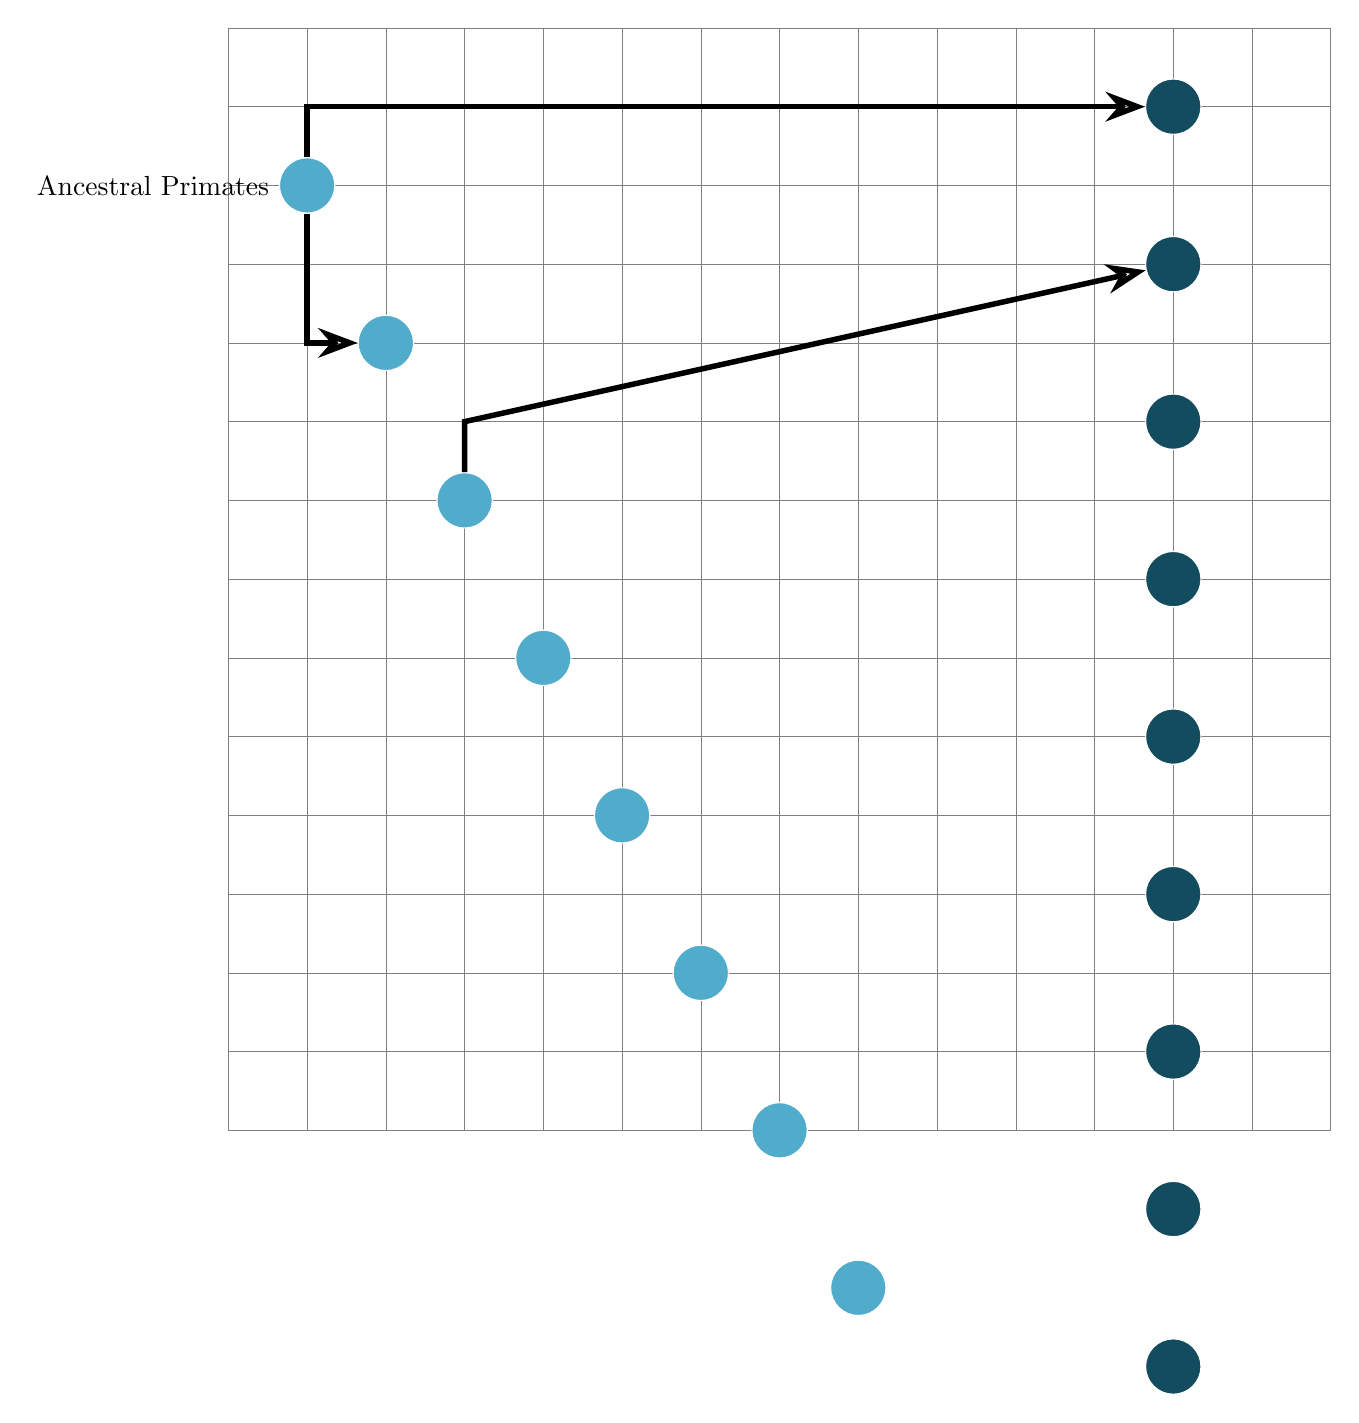
\begin{tikzpicture}
        [main/.style = {draw=white, text=black, circle, fill=bluedot,rounded corners=0.5mm,minimum size=2em},
        element/.style = {draw=white, text=black, circle, fill=darkblue,rounded corners=0.5mm,minimum size=2em},
        lines/.style = {line width=0.7mm, -{Stealth[length=5mm, open]}}]
        \draw[help lines] (-7,7) grid (7,-7); % Only for Development

        \node[main,label=left:{Ancestral Primates}] (R) at (-6,5) {};
        \node[main] (1) at (-5,3) {};
        \node[main] (2) at (-4,1) {};
        \node[main] (3) at (-3,-1) {};
        \node[main] (4) at (-2,-3) {};
        \node[main] (5) at (-1,-5) {};
        \node[main] (6) at (0,-7) {};
        \node[main] (7) at (1,-9) {};
        
        \node[element] (A) at (5,6) {};
        \node[element] (B) at (5,4) {};
        \node[element] (C) at (5,2) {};
        \node[element] (D) at (5,0) {};
        \node[element] (E) at (5,-2) {};
        \node[element] (F) at (5,-4) {};
        \node[element] (G) at (5,-6) {};
        \node[element] (H) at (5,-8) {};
        \node[element] (I) at (5,-10) {};

        \draw[lines] (R) -- (-6,6) -- (A); 
        \draw[lines] (R) -- (-6,3) -- (1); 
        
        \draw[lines] (2) -- (-4,2) -- (B); 


    \end{tikzpicture}
\end{center}

\end{document}